% Team Zenith -- Beyond Abstention (prototype: TrialGuide) -- group project proposal, v3
\documentclass[10pt,a4paper]{article}

% ---------------- layout and fonts ----------------
\usepackage[a4paper,left=1.65cm,right=1.65cm,top=1.45cm,bottom=1.55cm]{geometry}
\usepackage[T1]{fontenc}
\usepackage{mathptmx}
\usepackage{microtype}
\usepackage{amsmath,amssymb}
\usepackage{xcolor}
\usepackage{booktabs,tabularx,array}
\usepackage{enumitem}
\usepackage{titlesec}
\usepackage{tikz}
\usetikzlibrary{arrows.meta,positioning,shapes.geometric,fit,calc,backgrounds}
\usepackage{xurl}
\usepackage[hidelinks]{hyperref}
\usepackage{caption}
\usepackage{pifont}
\usepackage{float}

\definecolor{ink}{HTML}{1F2A37}
\definecolor{accent}{HTML}{1D4E89}
\definecolor{muted}{HTML}{5B6573}
\definecolor{tint}{HTML}{EEF3F9}
\definecolor{tint2}{HTML}{F6F7F9}
\definecolor{opt}{HTML}{FBF6EC}
\urlstyle{same}
\hypersetup{colorlinks=true,urlcolor=accent,linkcolor=accent,citecolor=accent}

\titleformat{\section}{\large\bfseries}{\thesection}{0.6em}{}
\titlespacing*{\section}{0pt}{7pt}{2.5pt}
\titleformat{\subsection}{\normalsize\bfseries}{\thesubsection}{0.5em}{}
\titlespacing*{\subsection}{0pt}{4pt}{1.5pt}
\setlist{nosep,leftmargin=1.15em}
\setlength{\parindent}{0pt}
\setlength{\parskip}{3pt}
\captionsetup{font=small,labelfont=bf,skip=2.5pt}
\setlength{\textfloatsep}{8pt}
\setlength{\intextsep}{6pt}
\newcolumntype{L}{>{\raggedright\arraybackslash}X}
\newcolumntype{P}[1]{>{\raggedright\arraybackslash}p{#1}}
\newcolumntype{C}[1]{>{\centering\arraybackslash}p{#1}}
\renewcommand{\arraystretch}{1.1}
\newcommand{\yes}{\ding{51}}
\newcommand{\no}{\textcolor{muted}{\ding{55}}}
\newcommand{\partly}{\textcolor{muted}{\(\sim\)}}

\tikzset{
  box/.style={draw=muted, rounded corners=2.5pt, align=center, fill=white, font=\footnotesize, inner sep=3pt},
  key/.style={box, draw=accent, line width=1pt, fill=tint},
  optb/.style={box, dashed, fill=opt},
  dec/.style={diamond, aspect=2.1, draw=accent, line width=1pt, fill=tint, align=center, inner sep=0.5pt, font=\footnotesize},
  arr/.style={-{Stealth[length=2mm]}, color=muted, line width=0.65pt},
  lab/.style={font=\scriptsize, color=muted},
  head/.style={font=\footnotesize\bfseries, color=accent}}

\begin{document}

% ---------------- title ----------------
\begin{center}
{\LARGE\bfseries Beyond Abstention: Risk-Controlled Inference and\\[2pt] Selective Clarification for Clinical Trial Matching}\\[4pt]
{\normalsize Prototype: \textbf{TrialGuide}}\\[5pt]
{\normalsize\bfseries Team Zenith}\\[2pt]
{\small
\begin{tabular}{@{}l@{\hspace{2.2em}}l@{}}
Prakash Bhabad, 2025204016 & Metta Venkata Ramana Murthy, 2025204034\\
\href{mailto:prakash.bhabad@students.iiit.ac.in}{prakash.bhabad@students.iiit.ac.in} & \href{mailto:metta.murthy@students.iiit.ac.in}{metta.murthy@students.iiit.ac.in}\\[1pt]
Prateek Singh, 2026701041 & Vidur Shah, 2026909004\\
\href{mailto:prateek.s@research.iiit.ac.in}{prateek.s@research.iiit.ac.in} & \href{mailto:vidur.shah@students.iiit.ac.in}{vidur.shah@students.iiit.ac.in}\\
\end{tabular}}\\[2pt]
{\small\itshape Language Models and Agents, Group Project Proposal, Monsoon 2026}
\end{center}

\vspace{-5pt}
\begin{center}
\fcolorbox{muted}{tint2}{\parbox{0.95\textwidth}{\small
\textbf{Summary.} LLM systems that check patients against clinical trial rules usually treat a rule the patient note does not settle in one of two ways: they abstain (``not enough information'') or they quietly fill the gap. We study a third option. For each unresolved rule, the system decides whether the note supports an \emph{inference}, whether a short \emph{question} to the doctor is worth asking because the answer would change the trial ranking, or whether it should \emph{abstain}. Inferences that could make an ineligible patient look eligible are only accepted below a target risk set by conformal risk control. Clinical trial matching is the test domain; the research question is about selective clarification and risk-controlled inference under a small question budget.}}
\end{center}
\vspace{-3pt}

% =====================================================================
\section{Introduction}
\textbf{Domain and target user.} Clinical trial recruitment. The user is a doctor or trial coordinator who wants a ranked shortlist of trials for a patient. TrialGuide only suggests; it has no way to enrol a patient, contact anyone or write to a record.

\textbf{Problem statement.} About 80\% of clinical trials miss their enrolment target or timeline, and finding eligible patients is the most common cause of delay~\cite{jmir}. Screening a patient means checking every inclusion and exclusion rule of many trials, which takes a clinician close to a minute per patient--trial pair~\cite{trialgpt}. LLM systems now automate this rule by rule; TrialGPT reaches 87.3\% rule-level accuracy with GPT-4~\cite{trialgpt}. When a note does not address a rule, TrialGPT labels it ``not enough information'', and in a manual analysis of 26 of its errors, 30.7\% were cases where the answer could have been inferred~\cite{trialgpt}. Other systems fill such gaps by inference~\cite{anesy} or flag them as unresolved~\cite{verdict}, but none asks the clinician only the questions that matter, and none controls how often a filled-in gap is wrong in the direction that matters most clinically. An error that makes an ineligible patient look eligible is more serious than one that hides a suitable trial, yet current evaluations count both the same.

\textbf{Goal.} Measure whether evidence-supported inference plus a few well-chosen questions can recover most of the trial ranking obtained with complete information, while keeping harmful inferences under a stated risk target, and compare this against fixed-order questioning, plain abstention and plain confidence thresholds.

\textbf{Expected contribution.} (1) A decision policy that, for each unresolved eligibility rule, chooses between evidence-supported inference, a clarifying question and abstention; (2) a conformal risk-control procedure for harmful inferences, with its assumptions and failure cases stated, compared against plain confidence thresholds; (3) ranking-aware question selection under a budget of three, compared against fixed-order and uncertainty-only selection; (4) a reproducible masked benchmark with a simulated clinician. To our knowledge no published trial-matching study combines these, but we claim the combination and its evaluation, not any single part.

% =====================================================================
\section{Background and Research Gap}
\textbf{What is solved.} TrialGPT~\cite{trialgpt} established rule-by-rule LLM matching with retrieval and ranking, close to expert accuracy on public benchmarks. Zero-shot matching on real notes has also been shown~\cite{wornow}. \textbf{What is partly addressed.} \(\alpha\)NeSy-CTM~\cite{anesy} infers missing facts by LLM abduction, and its authors note that this ``can overfill missing facts''; Verdict~\cite{verdict} marks rules as imputed or unresolved without closing them. \textbf{Related question-asking work.} MediQ~\cite{mediq} and ALFA~\cite{alfa} study follow-up questions for diagnosis; MediQ found that plain prompting to ask questions \emph{lowered} accuracy by 11.3\%, so asking only helps when it is selective. Feature-acquisition work~\cite{afa} chooses measurements for a top-\(k\) decision, but over gene-expression features rather than free-text rules and without a person in the loop. A 2025 survey describes interactive matching as ``largely absent'' from trial recruitment research~\cite{survey}.

\begin{table}[H]
\centering\footnotesize
\begin{tabularx}{\textwidth}{@{}P{3.3cm}P{2.6cm}C{1.55cm}C{1.55cm}C{1.9cm}L@{}}
\toprule
\textbf{Work} & \textbf{Task} & \textbf{Infers unstated facts} & \textbf{Asks a person} & \textbf{Controls error rate of inferences} & \textbf{How it treats an unresolved rule}\\
\midrule
TrialGPT~\cite{trialgpt} & Trial matching & \no & \no & \no & Abstains (``not enough information'')\\
\(\alpha\)NeSy-CTM~\cite{anesy} & Trial matching & \yes & \no & \no & Fills it by abduction\\
Verdict~\cite{verdict} & Trial matching & \partly & \no & \no & Marks it imputed or unresolved\\
MediQ~\cite{mediq}, ALFA~\cite{alfa} & Diagnosis & \no & \yes & \no & Asks; abstains on low confidence\\
Feature acquisition~\cite{afa} & Gene-based diagnosis & \no & \partly & \no & Acquires the most informative feature\\
\midrule
\textbf{This project} & \textbf{Trial matching} & \yes & \yes & \yes & \textbf{Infers, asks or abstains}\\
\bottomrule
\end{tabularx}
\caption{What prior work does with a rule the note does not settle. \(\sim\) = partly.}
\end{table}

\textbf{Selective clarification versus ordinary question answering.} In question answering the user asks and the model answers. Here the model decides \emph{whether} a question is worth one of a few slots, and \emph{which} one, judged by how much the answer could change a ranking over many trials, where one answer can settle the same rule in several trials. \textbf{The gap}, as far as we can find, is a trial-matching method that (i) separates evidence-supported inference from assumption, (ii) controls the rate of harmful inferences with a stated statistical procedure, and (iii) spends a small question budget where it changes the ranking most. We make no claim that any single ingredient is new; the contribution is the decision policy that combines them and its evaluation.

% =====================================================================
\section{What Counts as a Valid Inference}
Every rule the system handles is placed in one of four categories. Only the first two may be used as facts.

\begin{table}[H]
\centering\footnotesize
\begin{tabularx}{\textwidth}{@{}P{2.4cm}P{3.6cm}LP{2.6cm}@{}}
\toprule
\textbf{Category} & \textbf{Meaning} & \textbf{Example (rule \(\to\) note)} & \textbf{System action}\\
\midrule
Explicitly stated & The note says it directly & ``No prior chemotherapy'' \(\to\) ``She has never received chemotherapy'' & Use it; cite the sentence\\
Evidence-supported inference & Follows from stated facts by a rule or calculation a clinician would accept & ``eGFR \(\ge\) 60\,mL/min/1.73\,m\(^2\)'' \(\to\) 62-year-old woman, serum creatinine 1.9\,mg/dL; CKD-EPI 2021~\cite{ckdepi} (age, sex, creatinine) gives about 29, so not met. ``BMI \(\ge\) 30'' \(\to\) height 160\,cm, weight 82\,kg; BMI 32.0, so met. If any input is absent, the value is missing, not inferred & Use it if it passes risk control; cite the inputs and the tool output\\
Unsupported assumption & Plausible, but the note does not establish it & ``No prior chemotherapy'' \(\to\) ``newly diagnosed breast cancer''. Neoadjuvant treatment or an earlier cancer is still possible & Never used as a fact; becomes a candidate question\\
Missing & Nothing in the note bears on it & ``No hepatitis B'' \(\to\) not mentioned anywhere & Ask if it changes the ranking, otherwise abstain\\
\bottomrule
\end{tabularx}
\caption{Information categories. Two team members label 200 rule--note pairs with these categories to measure agreement (Cohen's \(\kappa\)) before the categories are used for evaluation.}
\label{tab:cat}
\end{table}

\textbf{Which errors matter more.} An inference is \emph{harmful} if it is wrong and moves the patient toward eligibility (an inclusion rule wrongly marked met, or an exclusion rule wrongly marked not met). At trial level we separate \emph{false-eligible} decisions (an ineligible patient shown as eligible; a safety risk) from \emph{false-exclusion} decisions (an eligible patient ruled out; a missed opportunity). Risk control is applied to the first kind; the second is reported and traded off, not ignored.

% =====================================================================
\section{Research Questions and Hypotheses}
\textbf{Main question.} Under a limited question budget, can evidence-supported inference and ranking-aware question selection recover more of the full-information trial ranking than fixed-order questioning or abstention, without increasing harmful inference? RQ1 and RQ2 are the core study. RQ3 is optional and runs only if time and compute allow. All thresholds below are fixed before any results.

\begin{table}[H]
\centering\footnotesize
\begin{tabularx}{\textwidth}{@{}P{1.25cm}P{3.9cm}LP{2.3cm}P{3.9cm}@{}}
\toprule
& \textbf{Question} & \textbf{Hypothesis and falsification} & \textbf{Comparison} & \textbf{Metrics and interpretation}\\
\midrule
\textbf{RQ1}\newline core & With at most 3 questions per patient, does the adaptive infer--ask--abstain policy recover more of the full-information ranking than fixed-order questioning and standard abstention? & \textbf{H1:} recovery (Eq.~\ref{eq:rec}) at least 10 points above fixed-order questioning, with a false-eligible rate no higher. Effect-size target: an estimated gain of \(\ge\)10 points; evidence: the paired 95\% CI. \emph{Supported} if the estimate is \(\ge\)10, the CI excludes zero and the false-eligible rate is not higher than B4's; \emph{not supported} if the CI's upper bound is below 10; \emph{inconclusive} otherwise. & B7 vs B4 and B6 (B2 as reference); budget sweep 0--5; ablations A1--A3 & Recovery, NDCG@10, P@10, false-eligible and false-exclusion rates, questions per patient. A gain that survives A1--A3 shows the policy, not the extra information, does the work.\\
\addlinespace
\textbf{RQ2}\newline core & What is the trade-off between inference coverage and harmful-inference risk, and does conformal risk control improve on conventional confidence thresholds? & \textbf{H2:} at \(\alpha=5\%\), on the fixed test split, the risk-controlled policy's harmful-inference rate is lower than that of a fixed 0.9 threshold and an uncorrected tuned threshold, and within \(\alpha\); useful coverage is reported alongside. \emph{Supported} if the upper 95\% bound of its rate is \(\le\alpha\); \emph{contradicted} if the lower bound is \(>\alpha\); \emph{inconclusive} if the interval crosses \(\alpha\). Resplits are exploratory only. & B5 (fixed and tuned thresholds) vs B7; \(\alpha\in\{2,5,10\}\%\) & Harmful-inference rate with CI, inference and useful coverage, accepted-inference count, abstention rate, risk--coverage curves, calibration error.\\
\addlinespace
\textbf{RQ3}\newline optional & How much of RQ1 and RQ2 performance is kept when the same framework runs on a QLoRA-tuned 8B open model? & \textbf{H3:} rule-level accuracy within 3 points of the 32B backbone and recovery within 5 points. \emph{False} if the lower 95\% bound of either gap is beyond these margins. Dropped if the core backbone itself falls back to 8B. & E1 vs core backbone; untuned 8B & Rule accuracy, recovery, harmful rate, cost and latency per patient.\\
\bottomrule
\end{tabularx}
\caption{Research questions mapped to hypotheses, comparisons and metrics. RQ1 refines the claim our team submitted for the Lecture~12 activity (same baseline, budget and 10-point target, now with three pre-set outcomes).}
\label{tab:rq}
\end{table}

% =====================================================================
\section{Method: the TrialGuide Decision Policy}
\begin{figure}[H]
\centering
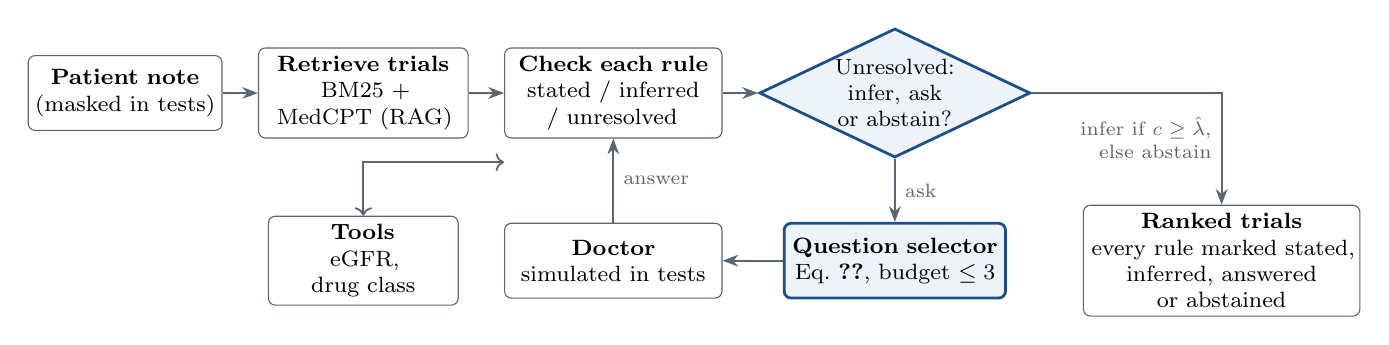
\begin{tikzpicture}
\node[box, text width=2.25cm, minimum height=0.95cm] (note) {\textbf{Patient note}\\(masked in tests)};
\node[box, text width=2.45cm, minimum height=0.95cm, right=0.45cm of note] (ret) {\textbf{Retrieve trials}\\BM25 + \mbox{MedCPT} (RAG)};
\node[box, text width=2.55cm, minimum height=0.95cm, right=0.45cm of ret] (chk) {\textbf{Check each rule}\\stated / inferred / unresolved};
\node[dec, right=0.45cm of chk] (pol) {Unresolved:\\infer, ask\\or abstain?};
\node[key, text width=2.6cm, minimum height=0.95cm, below=0.8cm of pol] (sel) {\textbf{Question selector}\\Eq.~\ref{eq:sel}, budget \(\le 3\)};
\node[box, text width=2.55cm, minimum height=0.95cm] (doc) at (chk |- sel) {\textbf{Doctor}\\simulated in tests};
\node[box, text width=2.2cm, minimum height=0.95cm] (tool) at (ret |- sel) {\textbf{Tools}\\eGFR, drug class};
\node[box, text width=3.3cm, minimum height=0.95cm] (out) at ($(sel)+(4.15,0)$) {\textbf{Ranked trials}\\every rule marked stated,\\inferred, answered or abstained};
\draw[arr] (note) -- (ret);
\draw[arr] (ret) -- (chk);
\draw[arr] (chk) -- (pol);
\draw[arr] (pol) -- node[lab, right]{ask} (sel);
\draw[arr] (sel) -- (doc);
\draw[arr] (doc) -- node[lab, right]{answer} (chk);
\draw[arr, <->] (tool.north) |- ([yshift=-3mm]chk.south west);
\draw[arr] (pol.east) -| node[lab, pos=0.7, left, align=right]{infer if \(c\ge\hat\lambda\),\\else abstain} (out.north);
\end{tikzpicture}
\caption{The decision loop. Every component sees only the visible part of the note; the simulated doctor is the only component that holds hidden facts. The highlighted parts are the contribution.}
\label{fig:loop}
\end{figure}

\textbf{Steps.} (1) Generate search keywords from the \emph{visible} note and retrieve candidate trials (BM25 + MedCPT~\cite{medcpt}, as in TrialGPT). (2) For each rule, the checker labels it stated, inferred or unresolved, gives the evidence sentence(s), and for an inference a confidence \(c\), computed as agreement across 5 sampled checks. Tools are called only for values that must be computed or looked up (eGFR, drug class~\cite{rxnav}). (3) An inference that moves the patient toward eligibility is accepted only if \(c \ge \hat\lambda\) (below); otherwise it becomes a candidate question. (4) Rules that depend on the same fact across trials are merged into one candidate. (5) The selector asks the highest-scoring candidate, re-checks only affected rules, re-ranks, and repeats until the budget is used or no candidate can change the top 10. (6) Remaining unresolved rules are reported as abstentions.

\textbf{Ranking-aware selection.} For a candidate fact \(f\) with possible answers \(a\), current trial scores \(s_t\), scores \(s_t^{f=a}\) if the answer were \(a\), current ranks \(r_t\), and the model's answer probabilities \(p(a)\):
\begin{equation}\label{eq:sel}
\mathrm{Score}(f)=\sum_{a}p(a)\sum_{t}\frac{\lvert s_t^{f=a}-s_t\rvert}{\log_2(1+r_t)}.
\end{equation}
Changes near the top weigh more, and facts shared by many trials score higher. Ablation A3 replaces this with uncertainty-only selection (ask the least certain rule regardless of its effect on the ranking). The probabilities \(p(a)\) are the model's guesses about the answer's value, used only to weigh possible ranking changes. They are not calibrated, and they say nothing about whether the doctor can actually answer from the records available. We therefore log every ``not documented'' reply and include high-impact but unanswerable questions in the failure analysis.

\subsection{Risk control: procedure, assumptions and limits}
\textbf{Unit and loss.} The unit of risk control is the \emph{patient}. For calibration patient \(i\) and threshold \(\lambda\), \(L_i(\lambda)\) is the number of harmful inferences accepted at confidence \(\ge\lambda\), divided by the number of that patient's unresolved rules across all candidate trials (\(L_i=0\) if there are none). \(L_i\in[0,1]\) and does not increase as \(\lambda\) rises. Using the patient as the unit keeps the many correlated rules of one patient from being counted as independent evidence.

\textbf{Calibration set and reference labels.} Calibration patients are disjoint from development and test patients, and the model, prompts and policy are frozen before calibration starts. Each calibration patient is masked with the same procedure, and independent seeds, as test patients. Whether an inference is harmful is judged against a reference rule status from one of two sources, which are never pooled in reporting: (a) \emph{expert labels}, the 1{,}020 TrialGPT rule annotations~\cite{trialgptann}; and (b) a \emph{model-derived reference}, the backbone's own judgement on the full note. Source (b) is not ground truth: it can share the system's blind spots, so errors common to both stay hidden. A 200-rule hand audit estimates its agreement with people but does not turn it into expert annotation. Primary harmful-inference claims use (a). If week 1 shows that expert labels cover too few calibration patients, calibration uses (b), and we say so; every risk result is then also reported on expert-labelled rules only, as a sensitivity analysis that excludes model-derived references. Results tables always label which setting a number comes from: calibrated and tested on expert labels; calibrated on model-derived references; or the expert-only sensitivity check. Only the first can be described as risk control against expert judgement, and none is described as a clinical safety guarantee.

\textbf{Threshold.} Following conformal risk control~\cite{crc}, with \(n\) calibration patients and target \(\alpha\),
\begin{equation}\label{eq:crc}
\hat\lambda=\inf\Big\{\lambda:\tfrac{n}{n+1}\hat R_n(\lambda)+\tfrac{1}{n+1}\le\alpha\Big\},\qquad \hat R_n(\lambda)=\tfrac1n\textstyle\sum_{i=1}^{n}L_i(\lambda).
\end{equation}
\textbf{What this gives, and what it does not.} Assumption: calibration and test patients are exchangeable, meaning they come from the same benchmark pool through one random patient-level split, are masked by the same procedure, and face the same frozen model and prompts. Under that assumption the \emph{expected} per-patient harmful-inference rate on a new patient is at most \(\alpha\), where the expectation is over calibration and test draws. This is an average statistical objective. It is not a safety guarantee for any single decision or patient, and it does not carry over to patients drawn differently (for example the optional Indian-affiliated set). \textbf{When the target cannot be met.} The smallest certifiable target is \(1/(n+1)\); with \(n=73\), \(\alpha=2\%\) needs a calibration rate below about 0.7\%. If no \(\lambda\) satisfies Eq.~\ref{eq:crc}, the system accepts no permissive inferences (it only asks or abstains), and we report the target as not achievable rather than relaxing it. This is why the pre-registered target is \(\alpha=5\%\), with 2\% and 10\% also reported. \textbf{Meeting the target is not the same as being useful.} The target can always be met by accepting almost nothing, so we also report \emph{useful coverage}: correct accepted inferences divided by unresolved rules. If the target is met with useful coverage below 10\%, we report it as met through near-total abstention, not as a practical success. The conformal guarantee is about expected risk under exchangeability; the test-set confidence interval describes uncertainty in one realised estimate. The two answer different questions and are reported separately. \textbf{Primary test evaluation.} \(\hat\lambda\) is computed once, on the calibration split, and applied unchanged to the fixed test split, which is opened once. Every risk estimate is reported with the number of patients contributing, the number of unresolved rules, the number of accepted inferences and the number judged harmful, the inference coverage and abstention rate, and a patient-level bootstrap 95\% CI. \textbf{Exploratory robustness.} Only after the primary results are frozen, we repeat the calibration/test split 200 times within the non-development patients to see how much the realised rate varies across splits. These resplits reuse test patients, so they are reported separately and never used to choose models, prompts or thresholds.

\subsection{Capabilities and why each is needed}
\begin{table}[H]
\centering\footnotesize
\begin{tabularx}{\textwidth}{@{}P{1.9cm}LP{5.4cm}@{}}
\toprule
\textbf{Capability} & \textbf{Role in the research question} & \textbf{Measured by}\\
\midrule
Reasoning (core) & Separates stated facts, evidence-supported inferences and assumptions (Table~\ref{tab:cat}); every inference carries evidence and a confidence. & Rule-level accuracy; inference precision on gold pairs; error breakdown by category\\
Agentic (core) & Decides per rule to infer, ask or abstain; tracks unresolved facts across trials; stops; hands the decision to the doctor. & Recovery vs questions; questions per patient; questions asked after the top 10 stopped changing\\
RAG (core) & Retrieves trials from the visible note; grounds inferences in cited sentences. & Recall of eligible trials; share of cited sentences found verbatim; ablation A4\\
Tool calling (supporting) & Computes values a model should not guess (eGFR from creatinine, drug class). & Correct tool and arguments; tool accuracy on 1{,}070 calculator items~\cite{ekacalc}; ablation A5; unsafe actions under planted prompts (target 0)\\
Fine-tuning (optional, E1) & Tests whether the policy survives on an 8B model a hospital could host. & RQ3 metrics\\
\bottomrule
\end{tabularx}
\caption{LLM capabilities, each tied to an evaluation. Fine-tuning is an optional extension, not part of the core claim.}
\end{table}

% =====================================================================
\section{Data, Masking and Leakage Control}\label{sec:data}
\begin{table}[H]
\centering\footnotesize
\begin{tabularx}{\textwidth}{@{}P{3.5cm}P{3.4cm}LP{2.1cm}@{}}
\toprule
\textbf{Source} & \textbf{Kind of label} & \textbf{Use} & \textbf{Licence / access}\\
\midrule
\href{https://www.trec-cds.org/2021.html}{TREC CT 2021} (75 pts), \href{https://www.trec-cds.org/2022.html}{2022} (50 pts) & Patient--trial: eligible / excluded / not relevant & Core: ranking, false-eligible and false-exclusion rates & Public research data\\
\href{https://data.csiro.au/collection/csiro:17152}{SIGIR 2016} (58 pts) & Patient--trial: eligible / potential / irrelevant & Core (ranking only) & CSIRO; terms to confirm\\
\href{https://huggingface.co/datasets/ncbi/TrialGPT-Criterion-Annotations}{TrialGPT annotations} & Patient--rule: expert label + evidence sentences, 1{,}020 rows & Core gold set for inference and harmful-inference & Public\\
\href{https://github.com/ncbi-nlp/TrialGPT}{TrialGPT code} & -- & Baseline pipeline and preprocessed trials & Public\\
\href{https://huggingface.co/datasets/ekacare/medical_calculator_eval}{Eka calculator set} & Calculator inputs and answers, 1{,}070 items & Tool accuracy & MIT\\
\href{https://pmc-patients.github.io/}{PMC-Patients}~\cite{pmcp} & None for trials (167{,}034 case-report summaries) & Optional: fine-tuning notes (E1); Indian-affiliated subset (E2) & CC BY-NC-SA\\
\href{https://clinicaltrials.gov/data-api/api}{ClinicalTrials.gov API}, \href{https://ctri.nic.in}{CTRI} & None & Optional E2: trials recruiting in India (605 on 2 Oct 2026) & Public\\
\bottomrule
\end{tabularx}
\caption{Data. The benchmark patients (183 in total) are expert-written synthetic descriptions. The \(>\)75{,}000 patient--trial judgements are trial-level labels, not 75{,}000 independently annotated clinical facts; only the 1{,}020 TrialGPT rows are expert labels at rule level.}
\end{table}

\textbf{Splits.} Patients are split once, at patient level: development 37 (prompt design, failure discovery, fine-tuning data), calibration 73 (risk control only) and test 73 (opened once). Patients that have expert rule annotations are kept in calibration and test so the gold evaluation stays clean; the exact count per split is checked in week 1. Trials are a shared corpus and appear across splits; no test patient--trial label is ever used for design, tuning or calibration.

\textbf{Masking.} Each note is split into single facts, then hidden in three ways: \emph{random} (40\% of facts in main runs; 20\% and 60\% for B4 and B7 only), \emph{rule-targeted} (facts that some candidate trial rule asks about) and \emph{evidence-targeted} on the gold pairs (exactly the sentences experts marked as evidence). Evidence-targeted masking gives a clean test: the correct response is known to be ``ask'' or ``abstain'' unless other visible text supports the answer, which two team members label.

\begin{figure}[H]
\centering
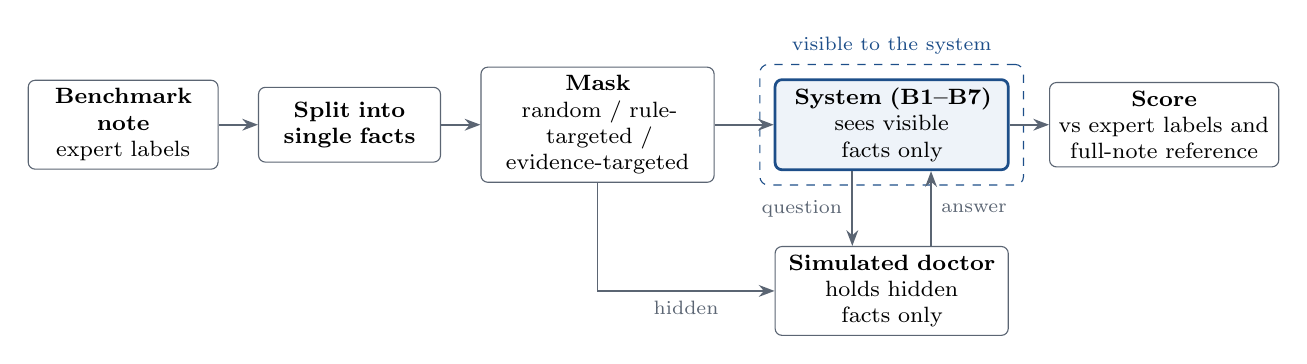
\begin{tikzpicture}
\node[box, text width=2.2cm, minimum height=0.95cm] (full) {\textbf{Benchmark note}\\expert labels};
\node[box, text width=2.1cm, minimum height=0.95cm, right=0.5cm of full] (facts) {\textbf{Split into}\\\textbf{single facts}};
\node[box, text width=2.75cm, minimum height=0.95cm, right=0.5cm of facts] (mask) {\textbf{Mask}\\random / rule-targeted /\\evidence-targeted};
\node[key, text width=2.75cm, minimum height=0.95cm, right=0.75cm of mask] (sys) {\textbf{System (B1--B7)}\\sees visible facts only};
\node[box, text width=2.7cm, minimum height=0.95cm, right=0.5cm of sys] (score) {\textbf{Score}\\vs expert labels and\\full-note reference};
\node[box, text width=2.75cm, minimum height=0.95cm, below=0.95cm of sys] (doc) {\textbf{Simulated doctor}\\holds hidden facts only};
\draw[arr] (full) -- (facts);
\draw[arr] (facts) -- (mask);
\draw[arr] (mask) -- (sys);
\draw[arr] (mask) |- node[lab, pos=0.75, below]{hidden} (doc);
\draw[arr] ([xshift=-5mm]sys.south) -- node[lab, left]{question} ([xshift=-5mm]doc.north);
\draw[arr] ([xshift=5mm]doc.north) -- node[lab, right]{answer} ([xshift=5mm]sys.south);
\draw[arr] (sys) -- (score);
\begin{scope}[on background layer]
\node[draw=accent, dashed, rounded corners=3pt, fit=(sys), inner sep=5pt, label={[lab, color=accent]above:visible to the system}] {};
\end{scope}
\end{tikzpicture}
\caption{Masking and visibility. Only the masked note crosses into the system boundary; hidden facts reach the system only as answers to the questions it chooses to ask.}
\label{fig:mask}
\end{figure}

\textbf{Leakage controls.} Keyword generation, retrieval, checking and selection see only the visible note; no patient or topic identifiers are passed to any model. TREC topics are public, so the model may have seen them during pretraining; we probe this by asking it to complete masked notes and by editing visible facts to check that inferences follow the text rather than memory, and report the result.

\textbf{Simulated doctor.} A model from a different family (Llama-3.1-8B-Instruct) answers each question only from the hidden facts, or says ``not documented'', adapted from the MediQ patient simulator~\cite{mediq}. Two team members check 150 answers for faithfulness (agreement reported). Simulated answers are cleaner than a real doctor's, so absolute recovery is an upper estimate; comparisons between policies use the same simulator and remain fair.

\textbf{Annotation protocol.} Four annotation tasks use people: information categories (200 rule--note pairs), evidence sufficiency on evidence-targeted masks, simulated-doctor faithfulness (150 answers) and the audit of model-derived references (200 rules). For each, a written guideline is drafted and piloted on development patients only and frozen at the end of week 2, before any calibration or test item is labelled. Two team members label every item independently and blind to system outputs; Cohen's \(\kappa\) is computed before any discussion; disagreements are settled by a third member whose decision and reason are logged. Test items are labelled after the freeze and are never used to change prompts, the policy or thresholds.

% =====================================================================
\section{Experimental Design}
\begin{table}[H]
\centering\footnotesize
\begin{tabularx}{\textwidth}{@{}P{0.6cm}P{4.6cm}P{4.3cm}L@{}}
\toprule
\textbf{ID} & \textbf{System} & \textbf{Component it isolates} & \textbf{Conclusion it supports}\\
\midrule
B1 & Full-information oracle (full note) & Upper bound & Ceiling for recovery\\
B2 & No question; infers with raw confidence, no risk control & Value of asking & Does clarification add anything?\\
B3 & Ask everything, no budget & Cost of full clarification & How many questions full recovery needs\\
B4 & Fixed-order questioning, budget 3 & Question selection & Main RQ1 comparison\\
B5 & Confidence-threshold inference (fixed 0.9; tuned without correction) & Risk control & Main RQ2 comparison\\
B6 & Standard abstention (TrialGPT-style; never infers, never asks) & Inference and asking together & Floor for recovery\\
B7 & \textbf{Adaptive infer--ask--abstain (ours)} & -- & --\\
\bottomrule
\end{tabularx}
\caption{Baselines. All use the same backbone model, patients, masks, retrieved trials and evidence, visibility rules, question budget (where applicable) and scoring code.}
\end{table}

\textbf{Ablations.} A1 without inference (ask or abstain only): how much comes from inference. A2 without adaptive selection (fixed order): how much comes from choosing questions. A3 uncertainty-only instead of ranking-aware selection: whether the ranking term in Eq.~\ref{eq:sel} matters. A4 without evidence retrieval: whether grounding inferences in cited text reduces harmful ones. A5 without tools: whether computed values reduce wrong inferences. A6 without risk control (raw confidence): what calibration buys. Sweeps over budget (0, 1, 2, 3, 5) and threshold \(\lambda\) give the recovery and risk--coverage curves.

\begin{equation}\label{eq:rec}
\text{Recovery}=\frac{\overline{\mathrm{NDCG@10}}_{\text{system}}-\overline{\mathrm{NDCG@10}}_{\text{B6}}}{\overline{\mathrm{NDCG@10}}_{\text{B1}}-\overline{\mathrm{NDCG@10}}_{\text{B6}}}
\end{equation}
NDCG@10 is computed per patient with the benchmark's graded labels, as in TrialGPT, and averaged over test patients (the bars). Recovery is the ratio of these averages, not an average of per-patient ratios, so a patient whose full-note and abstention rankings are nearly identical cannot produce a huge or undefined value. If the average gap between B1 and B6 in some slice is below 0.02, recovery is not reported for that slice and raw NDCG differences are shown instead. Uncertainty comes from a paired bootstrap over test patients that recomputes all three averages and the ratio in each resample; the 10-point threshold in H1 refers to this ratio.

\begin{table}[H]
\centering\footnotesize
\begin{tabularx}{\textwidth}{@{}P{4.1cm}LP{1.1cm}@{}}
\toprule
\textbf{Metric} & \textbf{Why it matters} & \textbf{RQ}\\
\midrule
NDCG@10, P@10, recovery & What the coordinator sees; comparable with TrialGPT & 1, 3\\
False-eligible rate & Ineligible patient shown as eligible: the safety-relevant error & 1, 2\\
False-exclusion rate & Eligible patient ruled out: a missed trial & 1, 2\\
Precision / recall of ``eligible'' & Trial-level decision quality, both directions & 1\\
Rule-level accuracy & Whether individual checks are right, on gold pairs & 1, 3\\
Harmful-inference rate (with CI) & The quantity risk control targets & 2\\
Inference coverage, useful coverage, accepted count & How much the policy infers, and how much of that is correct; exposes a target met by abstaining & 2\\
Abstention rate & How much is left to the doctor & 1, 2\\
Questions per patient & Doctor burden & 1\\
Recovery vs budget; risk--coverage curves; calibration error & Behaviour across operating points, not one number & 1, 2\\
\bottomrule
\end{tabularx}
\caption{Metrics. Errors toward eligibility and errors toward exclusion are always reported separately.}
\end{table}

\textbf{Statistics.} Paired bootstrap 95\% CIs over test patients for every headline metric; McNemar's test for paired rule-level and trial-level decisions; results per masking type, per budget and per rule type (demographic, lab value, diagnosis, prior treatment, comorbidity). Model names, versions and dates are logged for every run. The expert-labelled test subset may be small, so we report effect sizes with confidence intervals rather than relying on significance alone. A non-significant difference is not read as evidence of equivalence; the only equivalence-type claim is RQ3, which uses pre-set margins and confidence bounds. \textbf{Failure analysis.} Before building the full system we run a first version on the development patients, record every failure and group them; each group becomes a slice of the test report. The final report includes examples of correct inference, harmful inference, unnecessary questions, high-impact questions the doctor could not answer, appropriate abstention, and every case where the target risk could not be met. \textbf{Success criteria.} Results are judged on three separate dimensions, each against its own baselines, and are never combined into one overall score: (i) \emph{ranking recovery} (H1, against B4 and B6, across budgets); (ii) \emph{harmful-inference risk} with useful coverage (H2, against B5, on the fixed test split, with resplits as a separate robustness check); (iii) \emph{question burden} (questions per patient, the share answered ``not documented'', and recovery per question, against B3 and B4). Each dimension can succeed or fail on its own, and all three come with a failure analysis by rule type. A supported negative result, for example that adaptive selection does not beat fixed order, counts as a result.

% =====================================================================
\section{Optional Extensions}
\textbf{E1. Small open model (RQ3).} QLoRA (4-bit, rank 16)~\cite{qlora} on Qwen3-8B~\cite{qwen3}, trained on rule-level labels from the 32B backbone on development patients and PMC-Patients notes, kept only where they agree with the expert trial label and with a second sample. These are model-generated labels, not expert labels, and are reported as such. \textbf{E2. Indian-affiliated case reports.} PMC-Patients summaries whose source articles have authors at Indian institutions (PubMed affiliation metadata), oncology only, matched to trials recruiting in India. Author affiliation does not establish patient nationality or ethnicity, and published case reports over-represent unusual presentations and differ from routine records; the result is reported as an evaluation on Indian-affiliated case reports, with recalibration on part of the set. \textbf{E3. Clinician check.} If doctors agree to participate (not yet confirmed; ethics exemption to be confirmed with faculty), they label a small set and do a timed with/without comparison. \textbf{E4. More tools}, such as an Indian brand-to-generic drug lookup. The core study does not depend on any extension.

\section{Safety and Ethics}
Only public data is used: expert-written synthetic patients and published, de-identified case reports. TrialGuide has no tool that can enrol, contact or write; we plant instructions such as ``enrol this patient'' inside notes and count any attempt to act (target 0). Assumptions are never used as facts, every output lists what is unresolved, and the doctor makes every decision. Real hospital records are future work requiring ethics approval and a data-use agreement, and would be processed only by locally hosted models.

% =====================================================================
\section{Compute and Feasibility}
No paid API is needed. Core backbone: Qwen3-32B (4-bit, Apache 2.0) served with vLLM on Kaggle's free two-T4 sessions; simulated doctor: Llama-3.1-8B-Instruct. Kaggle currently gives about 30 GPU-hours per week per account, and the team has four accounts.

\begin{table}[H]
\centering\footnotesize
\begin{tabularx}{\textwidth}{@{}P{5.2cm}LP{2.0cm}@{}}
\toprule
\textbf{Job} & \textbf{Scale} & \textbf{GPU-hours (estimate)}\\
\midrule
Development runs and failure discovery & 37 patients, 2 masking types & \(\sim\)15\\
Full-note reference labels & 146 calibration + test patients \(\times\) 20 trials & \(\sim\)10\\
Calibration runs & 73 patients, shared checks cached & \(\sim\)20\\
Test runs, B1--B7 & 73 patients \(\times\) 3 masking types, \(\sim\)36K calls & \(\sim\)45\\
Ablations and sweeps & 40-patient subset, one masking type & \(\sim\)20\\
Simulated doctor & short calls & \(\sim\)5\\
\midrule
\textbf{Core total} & & \(\sim\)\textbf{115}\\
Optional E1 (teacher labels, QLoRA, evaluation) / E2 & & \(\sim\)60 / \(\sim\)20\\
\bottomrule
\end{tabularx}
\end{table}
\vspace{-3pt}
These figures are planning estimates, not measured performance. In week 1 we benchmark the 4-bit 32B model on 50 real rule-checking prompts: whether it fits in memory on two T4s with the context we need, prefill and decode speed, and the projected core GPU-hours. The decision rule is fixed now. If the model does not fit, or the projection exceeds about 200 GPU-hours, the whole core study (every baseline and the policy) switches to a smaller backbone from the same family (Qwen3-14B, then Qwen3-8B), so all comparisons still share one model. Further fallbacks are fewer masking types and a 40-patient subset for ablations. \textbf{Planned runs on the test split:} B1--B7 under three masking types (21 runs), random masking at 20\% and 60\% for B4 and B7 (4), budget sweep for B4 and B7 (10) and ablations A1--A6 (6), about 41 runs in total. Threshold sweeps, risk--coverage curves and resplits are recomputed from logged confidences and need no new model calls.

% =====================================================================
\section{Deliverables and Eight-Week Plan}
\begin{table}[H]
\centering\footnotesize
\begin{tabularx}{\textwidth}{@{}LL@{}}
\toprule
\textbf{Core (must finish)} & \textbf{Optional (if time and resources allow)}\\
\midrule
Dataset and leakage audit; split check; NEI count on gold pairs & E1 QLoRA 8B model (RQ3) and large-vs-small comparison\\
Reproduced TrialGPT-style baseline on the open backbone & E2 Indian-affiliated case-report evaluation with recalibration\\
Controlled masking protocol and simulated doctor with checks & E3 clinician labelling and timed comparison\\
Infer--ask--abstain policy with risk control; adaptive selection & E4 additional tools (Indian drug brands)\\
B1--B7 comparisons, risk--coverage evaluation, ablations A1--A6 & Short interactive demo\\
Failure analysis; reproducible prototype and released masked benchmark & \\
\bottomrule
\end{tabularx}
\end{table}
\vspace{-4pt}
\begin{table}[H]
\centering\footnotesize
\begin{tabularx}{\textwidth}{@{}P{0.9cm}L@{}}
\toprule
\textbf{Week} & \textbf{Work (core first; optional in italics)}\\
\midrule
1 & Data and leakage audit; splits fixed; count gold pairs per split and ``not enough information'' rate; 32B throughput and memory benchmark with go/no-go decision; TrialGPT-style baseline running\\
2 & Masking (three types) and simulated doctor; annotation guidelines piloted on development patients and frozen; memorisation probe\\
3 & Checker with evidence and tools; development failure analysis; B2, B4, B6 running\\
4 & Risk control and ranking-aware selection; B3, B5, B7; models and prompts frozen\\
5 & Calibration on the calibration split; ablations A1--A6 on development data; \emph{E1 teacher labels and QLoRA start}\\
6 & Annotation of calibration and test items; fixed test split opened once for RQ1 and RQ2; \emph{E2 data preparation}\\
7 & Statistics, error breakdown and case studies; exploratory resplit analysis after primary results are frozen; \emph{E1 evaluation (RQ3), E2 and E3 if available}\\
8 & Report and paper draft; code, masked benchmark and simulated doctor released\\
\bottomrule
\end{tabularx}
\end{table}

\section{Risks and Open Assumptions}
\begin{table}[H]
\centering\footnotesize
\begin{tabularx}{\textwidth}{@{}LL@{}}
\toprule
\textbf{Risk or assumption still to confirm} & \textbf{Plan}\\
\midrule
How many patients the 1{,}020 expert rows cover, and their split & Week 1 check; if too few for calibration, calibrate on the model-derived reference and report expert-only results as a sensitivity analysis\\
True rate of recoverable ``not enough information'' (TrialGPT's 30.7\% comes from 26 errors) & Measure on gold pairs in week 1; rule-targeted masking still creates realistic gaps\\
5\% target infeasible on calibration data & Report infeasibility and the smallest achievable \(\alpha\); policy falls back to ask/abstain\\
Backbone memorised public TREC patients & Memorisation probe; report; rely on evidence-targeted masking\\
SIGIR (CSIRO) and Kaggle drug-list licence terms & Confirm before use; drop the source if terms do not allow research use\\
Kaggle quota or 32B speed lower than estimated & Week 1 benchmark; switch the whole core study to Qwen3-14B or 8B by the fixed rule in Section~10\\
Doctor participation and ethics exemption & Only affects E3; core is unaffected\\
\bottomrule
\end{tabularx}
\end{table}

% ---------------- references ----------------
\vspace{-5pt}
{\footnotesize\raggedright
\begin{thebibliography}{99}\setlength{\itemsep}{0.3pt}
\bibitem{trialgpt} Q.~Jin et al. Matching patients to clinical trials with large language models. \emph{Nature Communications}, 2024. \url{https://www.nature.com/articles/s41467-024-53081-z}
\bibitem{trialgptann} TrialGPT criterion-level annotations. \url{https://huggingface.co/datasets/ncbi/TrialGPT-Criterion-Annotations}
\bibitem{anesy} Neurosymbolic clinical trial matching via LLM-driven abduction and logical verification, 2026. \url{https://arxiv.org/abs/2606.20895}
\bibitem{verdict} Accountable AI with grounded, faithful, consistent, actionable rationales: clinical trial matching with Verdict, 2026. \url{https://arxiv.org/html/2609.03366v1}
\bibitem{wornow} M.~Wornow et al. Zero-shot clinical trial patient matching with LLMs. \emph{NEJM AI}; arXiv 2024. \url{https://arxiv.org/abs/2402.05125}
\bibitem{mediq} S.~S.~Li et al. MediQ: question-asking LLMs and a benchmark for reliable interactive clinical reasoning. NeurIPS 2024. \url{https://arxiv.org/abs/2406.00922}
\bibitem{alfa} ALFA: aligning LLMs to ask good questions, a case study in clinical reasoning, 2025. \url{https://arxiv.org/abs/2502.14860}
\bibitem{afa} B.~Perets et al. Zero-shot active feature acquisition via LLM elicitation, 2026. \url{https://arxiv.org/abs/2606.18933}
\bibitem{survey} S.~Ghosh et al. A survey on LLM-assisted clinical trial recruitment. IJCNLP-AACL 2025. \url{https://aclanthology.org/2025.ijcnlp-long.35/}
\bibitem{jmir} M.~Br{\o}gger-Mikkelsen et al. Online patient recruitment in clinical trials: systematic review and meta-analysis. \emph{J Med Internet Res}, 2020. \url{https://pmc.ncbi.nlm.nih.gov/articles/PMC7673977/}
\bibitem{crc} A.~N.~Angelopoulos et al. Conformal risk control. ICLR 2024. \url{https://arxiv.org/abs/2208.02814}
\bibitem{medcpt} Q.~Jin et al. MedCPT. \url{https://github.com/ncbi/MedCPT}
\bibitem{rxnav} US National Library of Medicine. RxNav and RxClass APIs. \url{https://lhncbc.nlm.nih.gov/RxNav/APIs/}
\bibitem{ckdepi} L.~A.~Inker et al. New creatinine- and cystatin C-based equations to estimate GFR without race. \emph{NEJM}, 2021. \url{https://doi.org/10.1056/NEJMoa2102953}
\bibitem{ekacalc} Eka Care. Medical calculator evaluation set. \url{https://huggingface.co/datasets/ekacare/medical_calculator_eval}
\bibitem{pmcp} Z.~Zhao et al. A large-scale dataset of patient summaries for retrieval-based clinical decision support systems (PMC-Patients). \emph{Scientific Data}, 2023. \url{https://www.nature.com/articles/s41597-023-02814-8}
\bibitem{qlora} T.~Dettmers et al. QLoRA: efficient finetuning of quantized LLMs. NeurIPS 2023. \url{https://arxiv.org/abs/2305.14314}
\bibitem{qwen3} Qwen3 model cards. \url{https://huggingface.co/Qwen/Qwen3-32B}, \url{https://huggingface.co/Qwen/Qwen3-8B}
\end{thebibliography}}

\end{document}
